\documentclass[12pt, titlepage]{article}
\usepackage{float}
\usepackage{tabularx}
\usepackage{graphicx}
\usepackage{paralist}
\usepackage{listings}
\usepackage{booktabs}
\usepackage{hyperref}
\usepackage{amsfonts}
\usepackage{amsmath}
\usepackage{color}
\usepackage{fancyhdr}
\usepackage{geometry}
\geometry{margin = 0.75in}
\hypersetup{
    colorlinks,
    citecolor=blue,
    filecolor=black,
    linkcolor=red,
    urlcolor=blue
}
\usepackage[round]{natbib}

\begin{document}

\title{System Verification and Validation Plan for Digital Twin Forest} 
\author{Team 8, Forest Mirror\\Yichen Jiang\\ Bowen Zhang\\ Jiacheng Wu\\ Junhong Chen\\ Tingyu Shi}
\date{\today}
	
\maketitle

\pagenumbering{roman}

\section{Revision History}

\begin{tabularx}{\textwidth}{p{3cm}p{2cm}X}
\toprule {\bf Date} & {\bf Version} & {\bf Notes}\\
\midrule
October 29th & 1.0 & Initial Document\\
March 7th & 2.0 & Modify some test cases, finish Design Doc Verification
Plan\\
\bottomrule
\end{tabularx}

\newpage

\tableofcontents
\listoftables
\listoffigures

\newpage

\section{Symbols, Abbreviations and Acronyms}
The follow are some naming conventions and definitions from SRS:
\begin{itemize}
    \item LiDAR: Light Detection and Ranging(Scanning Technology)
    \item Plot: A square shaped area in the forest. There are 13 plots in
    total. 
    \item Target Forest: The natural forest modelled in this product.
    \item Digital Twin Forest: The virtual representation of the target
    forest.
    \item Update local data: The users are allowed to update any data on their
    own device. The update made by a user will not be updated to the other
    users.
    \item Update official data: The developing team would release updates
    regularly. The update made by the developing team can be updated to all
    users if they accept the latest version.
    \item Overall forest data: These are data for the whole forest. For
    example, these data may include overall $CO_2$ concentration or plant
    density of the whole forest.
    \item Forest plot data: The target forest is separated into 13 plots. Plot
    forest data has the same data types as the overall forest data, however,
    all the data are for a specific forest plot.
    \item Tree parameters: Tree parameters include data such as tree ages,
    perimeters, heights, species, etc.
    \item Main page: This is the first user interface when users just lunch the 
    system.
\end{itemize}
\newpage

\pagenumbering{arabic}
\section{General Information}

\subsection{Summary}
The software being tested is called \textit{Digital Twin Forest}. This isa
virtual representation of the target forest. The product will provide the 
following general functions:
\begin{itemize}
    \item Provide 3D models to simulate trees, soil, terrain, atmosphere, etc,
    in the target forest.
    \item Provide User Interface to present forest data(Overall forest
    data and Forest plot data) and tree parameters.
    \item Allow users to update local forest data and the virtual forest
    should present the changes.
    \item Allow users to update official data provided by the developing
    team.
\end{itemize}

\subsection{Objectives}

This document will perform as a guide of examining the quality of our software. The
first objective to be accomplished is to make sure correctness of the software.
Testing will allow our team to examine all the functions of our product. The software
should be executed properly, perform as designed, represent the expected data, and
show the model we constructed. The second objective is to examine the usability. The
possible methods might include manual testings by the testing team, questionnaires and
user interviews. 

\subsection{Relevant Documentation}
The System Verification Plan and Validation Plan mainly focuses 
on testing functional and non-functional requirements in the SRS documents. After the first 
submission of the SRS document, our team revised some SRS contents. You
can find the latest SRS document
\href{https://github.com/wuj187/DigitalTwinCAS/blob/main/docs/SRS/SRS.pdf}{\textcolor{red}{here}}. 

\section{Plan}
This section refers to the general testing plan of the project \textit{Digital Twin Forest}. 
To start with, it assigns different roles to the team members. Then, it contains the
SRS verification plan, which is divided into review by supervisor, reviewed by classmates
and reviewed by teammates. Then, it introduces the design verification which will be
completed later. This section also introduced how the team will test codes. Automated
testing tools are also given. Last, this section contains the plan for software
validation.

\subsection{Verification and Validation Team}
\begin{table}[H]
    \centering
    \begin{tabular}{|c|c|}
    \hline
         Team Member  & Roles\\
         \hline
         Yichen Jiang & Test leader\\
         \hline
         Bowen Zhang  & Hardware verification and SRS verification\\
         \hline
         Junhong Chen & Code verification\\
         \hline
         Jiacheng Chen & Code verification\\
         \hline
         Tingyu Shi & SRS verification and Code verification\\
         \hline
         Dr.Gonsamo & Manual testing as user\\
         \hline
         Dr.Gonsamo's lab's members  & Manual testing as users\\
         \hline
         Classmates & Manual testing as users\\
         \hline
    \end{tabular}
    \caption{Team Members and Roles}
\end{table}

\subsection{SRS Verification Plan}
SRS testing refers to the review the functional and non functional requirements mentioned
in the SRS document. In general, an SRS checklist will be created to verify if each
requirement has been met. The SRS may be revised by adding or removing requirements
based on new users' needs and constraints.

\subsubsection{Review by Supervisor}
The project is supervised by Dr. Gonsamo and his lab members. Our team meets weekly
with graduate students in Dr. Gonsamo's lab and reviews the progress of the project.
At the end of the semester, our team will have a formal meeting with Dr. Gonsamo, and
the project will be verified to see if it accomplishes all his expectations. 
Dr. Gonsamo will take the project and do a task-based inspection. For example, the application will be installed on lab computers and functions like measuring distance
between trees will be tested to see if it has an acceptable accuracy.

\subsubsection{Review by Classmates}
Classmates from other groups will be considered users who have no training
. Non-functional requirements in SRS can be tested by these reviewers, and
they will provide feedback. For example, it is clear that the application is
easy to learn if the reviewers successfully access the virtual forest in one minute.

\subsubsection{Review by teammates}
Team members are the reviewers who are most familiar with the project. The team will
go through the SRS document and carry out both system tests and unit tests. The SRS
checklist will be filled to see if all the functional and non-functional requirements
have been accomplished.

\subsection{Design Verification Plan}
Our design will be continuously improved with the implementation work heading on the final version. Our design will be discussed with our supervisor before, during and after we implement our product. The design will be modified according to the discussion with our supervisor and the advice given by course coordinator in the demonstrations within next months.

\subsection{Verification and Validation Plan Verification Plan}
The verification and validation plan verification plan aims at documenting how this verification and validation plan will be verified. The VnV plan will be reviewed by classmates from other groups and TAs and we will collect feedback and questions from them. The VnV plan will also be verified by the ForestMirror team when team members perform tests for the functional and non-functional requirements mentioned in SRS, and any modifications of the testing plans will be recorded. 



\subsection{Implementation Verification Plan}
Implementation verification refers to the high quality code of the application. Code
testing is mentioned in the system test description of this document, especially in
the tests for nonfunctional requirements. For example, a dynamic testing will be done
for performance requirements, and the team will perform individual code
walkthroughs. The team will follow the module guide and the traceability matrix to see
if the system follow low coupling and high cohesion principles
, another team member will help him/her do the
verification.
If the test fails, the code needs to be revised
before committing.\\
\noindent
Besides that, we will use static testing to ensure the code and documents are following good quality and our design. During the development, we will contact with our stakeholders to make sure we are doing the right products.

\subsection{Automated Testing and Verification Tools}

Automated testing tools, code coverage metrics, and linters have been mentioned in the
\href{https://github.com/wuj187/DigitalTwinCAS/blob/main/docs/DevelopmentPlan/DevelopmentPlan.pdf}{\textcolor{red}{development plan}}. \\
The team will use Visual Studio 2019 as the IDE of the project. The project is
implemented in C sharp language, and the built-in linter of VS2019 is good enough to
analyze the code and improve the quality. In VS2019, a unit test project of .NET
The framework that contains MSTest unit tests will be used for the unit testing. The
JetBrains dotCover will be installed as a plugin to check the code coverage. It can do
coverage analysis for the unit testing plan.

\subsection{Software Validation Plan}
Software validation is to guarantee SRS captures the right requirements.  As a
Meteorologist, Dr. Gonsamo, is not only the supervisor of the project but also a
stakeholder. As mentioned in the SRS verification section, Dr. Gonsamo will do a task-based inspection with the team. The functions of the application will be tested by trying to accomplish a range of task just to see if the requirements are necessary.

\newpage

\section{System Test Description}
\subsection{Tests for Functional Requirements}
The system tests about functional requirements
are divided into two subsets. The first subset is about 
testing presentations(what
contents will be presented to users). The second subset is about
testing if users can interact successfully with the product.
According to the newly revised SRS document mentioned in section 3.3, we have
18 functional requirements in total. The following are the
corresponding requirements within  two subsets
\begin{itemize}
    \item Presentation = \{FR1, FR4, FR5, FR9, FR12\}
    \item Users' interactions with the product = \{FR2, FR3, FR6, FR7, FR8
    FR10, FR11, FR13, FR14, FR15, FR16, FR17\}
\end{itemize}
\subsubsection{Presentation}
This section focuses on what contents are presented to users. 
From the SRS, there are 5 requirements related to the presentations, which
are FR1, FR4, FR5, FR9 and FR12. Each functional requirement will have at least one 
corresponding system test. The following are the system tests for requirements
related to presentations.

\begin{enumerate}
%%%%%%%%%%%%%%%%%%%%%%%%%%%%%% Test-FR1 %%%%%%%%%%%%%%%%%%%%%%%%%%%%%%%%%
\item{Test-FR1\\}
Control: Manual\\ 

Initial State: The product is just launched and running. Main page
is presented to users.\\

Input: A click event on \verb|Instruction| button on the main page.\\

Output: Instruction page will open and instructions about how to use 
the product will be presented in the instruction page.\\

Test Case Derivation: \verb|Instruction| button is designed for opening 
instruction page that contains instructions. Therefore, a click event on
\verb|Instruction| button will open instruction page.\\
					
How test will be performed: Let testers lunch the software and click on 
\verb|Instruction| button, instruction page with instructions should appear on the 
screen. After the instruction page has been displayed, testers set the system to the 
initial state(Main page) and retest the \verb|Instruction| button. Testers need to 
repeat this process 10 times.
%%%%%%%%%%%%%%%%%%%%%%%% Test-FR1 End %%%%%%%%%%%%%%%%%%%%%%%%%%%%%%%%%%%%%

%%%%%%%%%%%%%%%%%%%%%%%% Test-FR4.1 %%%%%%%%%%%%%%%%%%%%%%%%%%%%%%%%%%%%%%%%%
%% Test-FR4.1 will test from (main page --> overall forest view)
\item{Test-FR4.1\\}
Control: Manual\\ 

Initial State: The product is just launched and running. Main
page is presented to users.\\

Input: A click event for \verb|Start| button on the main page.\\

Output: A progress bar will appear on the screen to indicate how many
percentages of forest models are being loaded.\\

Test Case Derivation: Sometimes forest models can be large and they take
time to be loaded and presented to users. A progress bar can bring better
user experience to users by allowing them to know what is happening within the 
system. Clicking \verb|Start| will trigger the loading process of forest models.
While the forest models are being loaded, the progress bar should show on the screen.\\
					
How test will be performed: Let testers lunch the software and click on 
\verb|Start| button 10 times, the progress bar 
shall always appear on the screen after clicking
\verb|Start|.\\

\textcolor{red}{Forest models in this test case mean overall 
digital twin forest view.}
%%%%%%%%%%%%%%%%%%%%%%%% Test-FR4.1 End %%%%%%%%%%%%%%%%%%%%%%%%%%%%%%%%%%%%%%%

%%%%%%%%%%%%%%%%%%%%%%%% Test-FR4.2 %%%%%%%%%%%%%%%%%%%%%%%%%%%%%%%%%%%%%%%%%%%
%% Test-FR4.1 will test from (overall forest view --> a specific forest plot)
\item{Test-FR4.2\\}
Control: Manual\\ 

Initial State: The overall digital twin forest view with 14 plots 
and overall forest data is presented to users.\\

Input: A click event on any forest plot.\\

Output: A progress bar will appear on the screen to indicate how many
percentages of forest models are being loaded.\\

Test Case Derivation: Sometimes forest models can be large and they take
time to be loaded and presented to users. A progress bar can bring better
user experience to users by allowing them to know what is happening within the 
system. Clicking a specific forest plot will trigger the loading process of 
forest models. While the forest models are being loaded, the progress bar 
should show on the screen.\\
					
How test will be performed: Let testers click on each forest plots for 10 times(140 
times in total), the progress bar shall always appear on the screen after clicking
a forest plot.\\

\textcolor{red}{Forest models in this test case mean trees 
models within a specific forest plot.}
%%%%%%%%%%%%%%%%%%%%%%% Test-FR4.2 End %%%%%%%%%%%%%%%%%%%%%%%%%%%%%%%%%%%%%%%%

%%%%%%%%%%%%%%%%%%%%%%% Test-FR5 %%%%%%%%%%%%%%%%%%%%%%%%%%
\item{Test-FR5\\}
Control: Manual\\ 

Initial State: The product is just launched and running. Main page
is presented to users.\\

Input: A click event on \verb|Start| button on the main page.\\

Output: After the progress bar reaches 100\%, full view of overall digital 
twin forest is presented. Full view here includes 14 forest plots and overall forest
data. \\

Test Case Derivation: The product will present the digital twin forest in a 
hierarchical way. It will first display full view of the overall digital twin
forest. Then users can choose to display a specific forest plot. Therefore, after 
clicking \verb|Start|, full view of the overall digital twin forest should
appear on the screen after all the models are loaded. \\
					
How test will be performed: Let testers lunch the product and click \verb|Start| button
for 10 times, full view of the digital twin forest should always appear after the 
progress bar reaches 100\%. Also, testers need to make sure 14 forest plots and 
overall forest data can be displayed.

%%%%%%%%%%%%%%%%%%%% Test-FR5 End %%%%%%%%%%%%%%%%%%%%%%%%%

%%%%%%%%%%%%%%%%%%%%%%% Test-FR9.1 %%%%%%%%%%%%%%%%%%%%%%%%%%
\item{Test-FR9.1\\}
Control: Manual\\ 

Initial State: The forest model is presented to users and 
environmental data are not displayed.\\

Input: A click event on \verb|Environmental Data| button.\\

Output: Environmental data should appear on the left side of the 
screen.\\

Test Case Derivation: Environmental data are designed to be placed
on the left side of the screen. This can leave the center part 
of the screen to allow users to view the forest model.\\
					
How test will be performed: Let testers click 
\verb|Environmental Data| button 10 times. After each click, testers 
should reset the system to the initial state. Environmental data 
should display on the left side of the screen 10 times.
%%%%%%%%%%%%%%%%%%%% Test-FR9.1 End %%%%%%%%%%%%%%%%%%%%%%%%%

%%%%%%%%%%%%%%%%%%% Test-FR9.2 %%%%%%%%%%%%%%%%%%%%%%%%%%%%%%%
\item{Test-FR9.2\\}
Control: Manual\\ 

Initial State: The forest model is presented to users and 
tree parameters are not displayed.\\

Input: A click event on \verb|Tree Parameters| button.\\

Output: Tree parameters should appear on the right side of the 
screen.\\

Test Case Derivation: Tree parameters are designed to be placed
on the right side of the screen. This can leave the center part 
of the screen to allow users to view the forest model.\\
					
How test will be performed: Let testers click 
\verb|Tree Parameters| button 10 times. After each click, testers 
should reset the system to the initial state. Tree parameters
should display on the right side of the screen 10 times.
%%%%%%%%%%%%%%% Test-FR9.2 End %%%%%%%%%%%%%%%%%%%%%%%%%%%%%%%

%%%%%%%%%%%%%%% Test-FR12.1 %%%%%%%%%%%%%%%%%%%%%%%%%%%%%%%%%%
\item{Test-FR12.1\\}
Control: Manual\\ 

Initial State: Environmental data are presented.\\

Input: Testers record all the environmental data.\\

Output: N/A\\

Test Case Derivation: Since this test does not have any output, this 
part is not applicable.\\
					
How test will be performed: Let testers observe and record all the 
environmental data. Then testers need to check if the data observed
from the UI are exactly the same as data stored in the software. 
If data observed are the same as data stored in the UI, test passes.
Otherwise test fails. Testers can check the JSON files stored 
\href{https://github.com/tingyushi/DTForest-DS}{here}
as the data to be compared against. 
%%%%%%%%%%%%%%% Test-FR12.1 End %%%%%%%%%%%%%%%%%%%%%%%%%%%%%%

%%%%%%%%%%%%%%% Test-FR12.2 %%%%%%%%%%%%%%%%%%%%%%%%%%%%%%%%%%
\item{Test-FR12.2\\}
Control: Manual\\ 

Initial State: Tree parameters are presented.\\

Input: Testers record all the tree parameters.\\

Output: N/A\\

Test Case Derivation: Since this test does not have any output, this part is
not applicable.\\
					
How test will be performed: Let testers observe and record all the 
tree parameters. Then testers need to check if the data observed
from the UI are exactly the same as data stored in the software. 
If data observed are the same as data stored in the UI, test passes.
Otherwise test fails. Testers can check the JSON files stored 
\href{https://github.com/tingyushi/DTForest-DS}{here}
as the data to be compared against. 
%%%%%%%%%%%%%%% Test-FR12.2 End %%%%%%%%%%%%%%%%%%%%%%%%%%%%%%


\end{enumerate}

\subsubsection{Users' interactions with the product}
This section focuses on users' interactions with the system. 
From the SRS, there are 13 requirements related to users' interactions
with the system, which
are FR2, FR3, FR6, FR7, FR8, FR10, FR11, FR13, FR14, FR15, FR16, FR17 and FR18.
Each functional requirement will have at least one 
corresponding system test. The following are the system tests for requirements
related to users' interactions with the system.

\begin{enumerate}
 %%%%%%%%%%%%%%% Test-FR23 %%%%%%%%%%%%%%%%%%%%%%%%%%%%%%%%%%
\item{Test-FR2\&3\\}
Control: Manual\\ 

Initial State: The product is launched and running. Main page is
presented to users.\\

Input: A click event on \verb|Start| button.\\

Output: The screen should change from the main page
interface to the view of the forest model. \\

Test Case Derivation: If clicking \verb|Start| button can change the 
main page to the forest model view. Then we can prove that \verb|Start|
button provides a way to allow users to start the virtual tour of the 
digital twin forest.\\
					
How test will be performed:  Let testers launch the product and click 
\verb|Start| button 10 times, forest model view should always appear.
After forest model appeared, testers should reset the system to the 
initial state, which is the main page.
%%%%%%%%%%%%%%% Test-FR23 End %%%%%%%%%%%%%%%%%%%%%%%%%%%%%%

%%%%%%%%%%%%%%% Test-FR6.1 %%%%%%%%%%%%%%%%%%%%%%%%%%%%%%%%%%
\item{Test-FR6.1\\}
Control: Manual\\ 

Initial State: Environmental data are displayed.\\

Input: A click event on \verb|Environmental Data| button.\\

Output: Environmental data display should disappear from the screen.\\

Test Case Derivation: If environment data can disappear from the 
screen, this proves that data GUI can be minimized.\\
     
How test will be performed: Let testers click 
\verb|Environmental Data| button 10 times when environmental data 
are displayed, environmental data display should disappear 10 times.
After each click, testers need to reset the system to the initial 
state.
%%%%%%%%%%%%%%% Test-FR6.1 End %%%%%%%%%%%%%%%%%%%%%%%%%%%%%%

%%%%%%%%%%%%%%% Test-FR6.2 %%%%%%%%%%%%%%%%%%%%%%%%%%%%%%%%%%
\item{Test-FR6.2\\}
Control: Manual\\ 

Initial State: Tree parameters are displayed.\\

Input: A click event on \verb|Tree Parameters| button.\\

Output: Tree parameters display should disappear from the screen.\\

Test Case Derivation: If tree parameters can disappear from the 
screen, this proves that data GUI can be minimized.\\
     
How test will be performed: Let testers click 
\verb|Tree Parameters| button 10 times when tree parameters 
are displayed, tree parameters display should disappear 10 times.
After each click, testers need to reset the system to the initial 
state.
%%%%%%%%%%%%%%% Test-FR6.2 End %%%%%%%%%%%%%%%%%%%%%%%%%%%%%%

%%%%%%%%%%%%%%% Test-FR7 %%%%%%%%%%%%%%%%%%%%%%%%%%%%%%%%%%
\item{Test-FR7\\}
Control: Manual\\ 

Initial State: Overall digital twin forest view is presented. This view includes
14 forest plots and overall forest data.\\

Input: A click event on any forest plot.\\

Output: Windows to present forest plot data should appear on two sides of the 
screen.\\

Test Case Derivation: If clicking any forest plot can make windows to present forest
plot data appear on two sides of the screen. Then we can prove that the system is able
to present forest plot data.\\
					
How test will be performed:  Let testers click each forest plot for 10 times(140 times
in total), windows to present forest plot data should always appear on two sides of
the screen.
%%%%%%%%%%%%%%% Test-FR7 End %%%%%%%%%%%%%%%%%%%%%%%%%%%%%%

%%%%%%%%%%%%%%% Test-FR8 %%%%%%%%%%%%%%%%%%%%%%%%%%%%%%%%%%
\item{Test-FR8\\}
Control: Manual\\ 

Initial State: Various tree models are presented on the screen.\\

Input: A click event on any tree model.\\

Output: A pop-up window should appear to show related tree parameters.\\

Test Case Derivation: If clicking any tree model can make pop-up windows to present 
tree parameters appear on the screen. Then we can prove that the system is able
to present tree parameters.\\
					
How test will be performed:  Let testers randomly select 20 trees in each forest plot.
Since there are 14 forest plots, 280 trees will be selected in total. By clicking on
each tree, a pop-up window should always appear on the screen to show tree parameters.
%%%%%%%%%%%%%%% Test-FR8 End %%%%%%%%%%%%%%%%%%%%%%%%%%%%%%

%%%%%%%%%%%%%%% Test-FR10 %%%%%%%%%%%%%%%%%%%%%%%%%%%%%%%%%%
\item{Test-FR10\\}
Control: Manual\\ 

Initial State: Various tree models are presented on the screen.\\

Input: Testers press \verb|W| key and \verb|S| key.\\

Output: Tree models are zoomed in by pressing \verb|W| key, and zoomed out
by pressing \verb|S| key.\\

Test Case Derivation: In Unity, we can program \verb|W| and \verb|S| keys so that 
they can control the camera to move forward and move backward. If the camera moves
forward, which means getting closer to tree models, tree models are zoomed in 
equivalently. If the camera moves backward, which means getting further to tree 
models, tree models are zoomed out equivalently.\\
					
How test will be performed: Let testers press \verb|W| key 5 times in succession 
and each key press should last 2 seconds. Tree models should be zoomed in after 
each key press. After this, let testers press \verb|S| key 5 times in succession,
and each key press should last 2 seconds. Tree models should be zoomed out after
each key press.
%%%%%%%%%%%%%%% Test-FR10 End %%%%%%%%%%%%%%%%%%%%%%%%%%%%%%

%%%%%%%%%%%%%%% Test-FR11.1 %%%%%%%%%%%%%%%%%%%%%%%%%%%%%%%%%%
\item{Test-FR11.1\\}
Control: Manual\\ 

Initial State: The forest model is presented on the screen.\\

Input: Testers press \verb|A| key and \verb|D| key.\\

Output: Users' first view should move left after pressing \verb|A| key. Users'
first view should move right after press \verb|D| key.\\

Test Case Derivation: In Unity, we can program \verb|A| and \verb|D| keys so that 
they can control the camera to move left and move right. If the camera's position 
can change, user's point of view can also change.\\
					
How test will be performed: Let testers press \verb|A| key 5 times in succession 
and each key press should last 2 seconds.  The user's point of view should move left
after each key press. After this, let testers press \verb|D| key 5 times in 
succession, and each key press should last 2 seconds. The user's point of view 
should move right after each key press.
%%%%%%%%%%%%%%% Test-FR11.1 End %%%%%%%%%%%%%%%%%%%%%%%%%%%%%%

%%%%%%%%%%%%%%% Test-FR11.2 %%%%%%%%%%%%%%%%%%%%%%%%%%%%%%%%%%
\item{Test-FR11.2\\}
Control: Manual\\ 

Initial State: The forest model is presented on the screen.\\

Input: Users move the mouse in 4 different directions, which are left, right, 
forward, and backward.\\

Output:
\begin{itemize}
    \item Move the mouse forward: The user's first point of view should rotate up.
    \item Move the mouse backward: The user's first point of view should rotate 
    down.
    \item Move the mouse left: The user's first point of view should rotate left.
    \item Move the mouse right: The user's first point of view should rotate right.
\end{itemize}

Test Case Derivation: In Unity, the mouse can be programmed to adjust the 
angle of the camera. Therefore,  moving the mouse can change the point of view.\\
					
How test will be performed: \\ The test will be performed in 4 steps:
\begin{enumerate}[1.]
    \item Let testers move the mouse left, the point of view should rotate left.
    \item Let testers move the mouse right, the point of view should rotate right.
    \item Let testers move the mouse forward, the point of view should rotate up.
    \item Let testers move the mouse backward, the point of view should rotate down.
\end{enumerate}
%%%%%%%%%%%%%%% Test-FR11.2 End %%%%%%%%%%%%%%%%%%%%%%%%%%%%%%

%%%%%%%%%%%%%%% Test-FR13.1 %%%%%%%%%%%%%%%%%%%%%%%%%%%%%%%%%%
\item{Test-FR13.1\\}
Control: Manual\\ 

Initial State: Environmental data are displayed.\\

Input: A click event on \verb|turn page| button. A sample \verb|turn page| button
can be found in \textcolor{red}{section 7.3}.\\

Output: A pie chart indicating percentages of different tree types
should appear in the same window.\\

Test Case Derivation: \verb|Turn page| button is designed for turning pages, so 
clicking \verb|turn page| button should make a new page appear in the same window.
If a new page can appear on the screen by clicking \verb|turn page| button, then we 
can prove that the product allows users to turn pages if the interface has multiple
pages.\\
					
How test will be performed: Let testers click \verb|turn page| button on the 
window showing environmental data 10 times. The pie chart should
appear in the same window 10 times. 
Meanwhile, before each click, testers need to reset the system to the initial state.
%%%%%%%%%%%%%%% Test-FR13.1 End %%%%%%%%%%%%%%%%%%%%%%%%%%%%%%

%%%%%%%%%%%%%%% Test-FR13.2 %%%%%%%%%%%%%%%%%%%%%%%%%%%%%%%%%%
\item{Test-FR13.2\\}
Control: Manual\\ 

Initial State: Tree parameters are displayed.\\

Input: A click event on \verb|turn page| button. A sample \verb|turn page| button
can be found in \textcolor{red}{section 7.3}.\\

Output: Leaf information should appear in the same window.\\

Test Case Derivation: \verb|Turn page| button is designed for turning pages, so 
clicking \verb|turn page| button should make a new page appear in the same window.
If a new page can appear on the screen by clicking \verb|turn page| button, then we 
can prove that the product allows users to turn pages if the interface has multiple
pages.\\
					
How test will be performed: Let testers click \verb|turn page| button on the 
window showing tree parameters 10 times. Leaf information should appear in the same 
window 10 times. Meanwhile, before each click, testers need to reset the system to 
the initial state.
%%%%%%%%%%%%%%% Test-FR13.2 End %%%%%%%%%%%%%%%%%%%%%%%%%%%%%%

%%%%%%%%%%%%%%% Test-FR14 %%%%%%%%%%%%%%%%%%%%%%%%%%%%%%%%%%
\item{Test-FR14\\}
Control: Manual\\ 

Initial State: A forest plot view is presented to users.\\

Input: A click event on \verb|Back| button located at the left bottom of the screen.\\

Output: Overall view of digital twin forest should appear on the screen.\\

Test Case Derivation: \verb|Back| button is designed for returning to the 
previous user interface, so clicking \verb|Back| button should show overall digital
twin forest view. \\
					
How test will be performed:  Let testers click \verb|Back| button located at the left 
bottom of the screen when they are viewing forest plot models. After clicking \verb|Back|
button, overall digital twin forest should appear on the screen. 
This test should be done for 14 forest plots.
%%%%%%%%%%%%%%% Test-FR14 End %%%%%%%%%%%%%%%%%%%%%%%%%%%%%%

%%%%%%%%%%%%%%% Test-FR15 %%%%%%%%%%%%%%%%%%%%%%%%%%%%%%%%%%
\item{Test-FR15\\}
Control: Manual\\ 

Initial State: Main page is presented to users.\\

Input: A click event on \verb|Quit| button.\\

Output: Software should close.\\

Test Case Derivation: \verb|Quit| button is designed for quitting the software,
so clicking \verb|Quit| button quit the software.\\
					
How test will be performed:  Let testers click \verb|Quit| button located in the main
page. After clicking \verb|Quit| button, the software should close.
%%%%%%%%%%%%%%% Test-FR15 End %%%%%%%%%%%%%%%%%%%%%%%%%%%%%%

%%%%%%%%%%%%%%% Test-FR16 %%%%%%%%%%%%%%%%%%%%%%%%%%%%%%%%%%
\item{Test-FR16\\}
Control: Manual\\ 

Initial State: Update data page is presented.\\

Input: Testers enter new data in the input box and click \verb|Update| Button\\

Output: A text should pop up indicating if the update was successful.\\

Test Case Derivation: N/A.\\
					
How test will be performed: \\ The test will be performed in the following ways:
\begin{enumerate}[1.]
\item Testers select a plot.
\item Testers select updating environmental data or tree parameters. (If testers
choose to update tree parameters, testers also need to choose a tree type.)
\item Testers select the data type.
\item Testers enter the new data.
\item Testers press \verb|Update| button.
\item Testers should enter the forest model to check if the newly updated data can 
appear in the environmental data display or tree parameters display. 
\item Repeat the above steps for all 14 plots and 7 tree types.
\end{enumerate}
%%%%%%%%%%%%%%% Test-FR16 End %%%%%%%%%%%%%%%%%%%%%%%%%%%%%%

%%%%%%%%%%%%%%% Test-FR17 %%%%%%%%%%%%%%%%%%%%%%%%%%%%%%%%%%
\item{Test-FR17\\}
Control: Manual\\ 

Initial State: New version of the software is not downloaded.\\

Input: Users go to GitHub to download the new version.\\

Output: A new version product should be ready to use.\\

Test Case Derivation: Newly released version of Digital Twin Forest will be released
on GitHub. If users want to use the new version of the product with latest forest data
or some new features/functions, they can go to GitHub to download.\\
					
How test will be performed:  Let testers go to GitHub and download a new version.
The downloaded new version of the software should work properly.
%%%%%%%%%%%%%%% Test-FR17 End %%%%%%%%%%%%%%%%%%%%%%%%%%%%%%
\end{enumerate}


\subsection{Tests for Nonfunctional Requirements}

\subsubsection{Look and Feel Requirement testing}

\begin{enumerate}

\item{Test-NFR-LF1.1\\}

Type: Static.\\
How test will be performed: Testers open the Module Guide document and check the Traceability Matrix to see if each function trace over 8 modules.\\\\
Expected result: Each function trace over 8 modules.					
\item{Test-NFR-LF1.2\\}

Type: Static\\

How test will be performed: We will conduct interview random people for the feedback by providing the questionnaire in the Appendix, over 80 percent of the users answer the forest is lifelike.\\

Expected result: Over 80 percent of the users choose A or B in the first question in the questionnaire.

\item{Test-NFR-LF2.1\\}

Type: Static\\

How test will be performed: Testers will collect all the data and parameters of our forest and compare the data to the physical measurements. After that calculate the relative error of the data\\

Expected result: All environmental data and tree parameters have relative errors less than 0.1 comparing to the actual data our clients provide us.

\item{Test-NFR-LF2.2\\}

Type: Static\\

How test will be performed: We will conduct interview random people for the feedback by providing the questionnaire in the Appendix, over 80 percent of the users answer the system look professional.\\

Expected result: Over 80 percent of the users choose A or B in the second question in the questionnaire.

\subsubsection{Usability and Humanity Requirements testing}
\item{Test-NFR-UH1.1\\}

Type: Static\\

How test will be performed:  We will conduct interview random people for the feedback by providing the questionnaire in the Appendix, over 80 percent of the users answer the instructions are easy.\\

Expected result: Over 80 percent of the users choose A or B in the third question in the questionnaire.

\item{Test-NFR-UH2.1\\}

Type: Manual\\

Initial State: The system is launched\\

Input: Testers inspect all the texts on every UI component in the software \\

Result: All of the texts are in English.\\

How test will be performed: Testers open the software and inspect all the components containing texts in the software. 100 percent of the texts should be used in English.

\item{Test-NFR-UH3.1\\}

Type: Manual\\

Initial State: The system is launched and it is in the main page.\\

Input: A click event is made on the instructions option\\

Output: Instructions are displayed after the event\\

How test will be performed: Testers click on the instruction option and observe the response. Instructions are displayed on the screen.

\item{Test-NFR-UH4.1\\}

Type: Static\\

How test will be performed: We will conduct interview random people for the feedback by providing the questionnaire in the Appendix, over 80 percent of the users answer they notice and understand all the icons.\\

Expected result: Over 80 percent of the users choose A or B in the fourth question in the questionnaire.

\item{Test-NFR-UH4.2\\}

Type: Static\\

How test will be performed: We will conduct interview random people for the feedback by providing the questionnaire in the Appendix, over 80 percent of the users answer they think the icons used in the software are appealing.\\

Expected result: Over 80 percent of the users choose A or B in the fifth question in the questionnaire.

\item{Test-NFR-UH5.1\\}

Type: Manual\\

Initial State: The system is launched\\

Input: Input from mouse and keyboard from users\\

Output: All interactive components like button and sliding bar can be used normally by mouse and keyboard.\\

How test will be performed: Testers open the software and try to access all the interactive components in the software using a mouse and keyboard. Testers should end up completing all the actions without any trouble.

\item{Test-NFR-UH5.2\\}

Type: Static\\

How test will be performed: We will conduct interview random people for the feedback by providing the questionnaire in the Appendix, over 80 percent of the users answer they can learn how to use the system within half an hour.\\

Expected result: Over 80 percent of the users choose A or B in the sixth question in the questionnaire.

\subsubsection{Performance Requirements}
\item{Test-NFR-PR1.1\\}

Type: Manual\\

Initial State: The system is launched\\

Input: Input from mouse or keyboard to make an action in the application\\

Output: The system handles all the inputs from mouse or keyboard within 2 seconds\\

How test will be performed: Testers open the system and give input to the system. For example, the tester clicks the start button. The system should respond to any request within 2 seconds.

\item{Test-NFR-PR1.2\\}

Type: Manual\\

Initial State: The system is launched and goes to forest page\\

Input: None\\

Output: The system is running at over 30 FPS for 90 percent of the time\\

How test will be performed:  The system should run at over 30 FPS for 90 percent of the time in the forest page.

\item{Test-NFR-PR1.3\\}

Type: Manual\\

Initial State: The system is launched and the system is in main page\\

Input: A click event is triggered on the start option\\

Output: The system loads all the models within 10 seconds\\

How test will be performed: Testers open the system and click the start option, the testers should wait for less than 10 seconds for the models to show up.

\item{Test-NFR-PR3.1\\}

Type: Static\\

How test will be performed: Testers will record all the data and parameters in the system and compare the data to the physical measurements. After that, testers calculate the relative error of the data\\

Expected result: All the data of the forest have relative errors less than 0.1.

\item{Test-NFR-PR4.1\\}

Type: Manual\\

Initial State: System is not opened\\

Input: Testers give inputs to open the system\\

Output:The system opens normally 100 percent of the time\\

How test will be performed: Testers open the system and observe the system. the system should open normally 100 percent of the time.

\item{Test-NFR-PR4.2\\}

Type: Manual\\

Initial State: The system is launched\\

Input: Screen recording to record the system\\

Output: The system is working normally 24 hours a day\\

How test will be performed: Testers open the system and run the application in the background for 24 hours.

\item{Test-NFR-PR5.1\\}

Type: Manual\\

Initial State: The system is launched without an internet connection\\

Input: Testers give inputs for different actions\\

Output: The system responds to all the input actions normally\\

How test will be performed: Testers open the system without an internet connection. Testers do different actions in the system and see if the system responds normally, the system should finish 100 percent of the actions without any error.


\item{Test-NFR-PR6.1\\}

Type: Static\\

How test will be performed: Testers will assess the size of the system after the system is implemented\\

Expected result: The size of the software is less than 10 GB.

\subsubsection{Operational and Environmental Requirements}
\item{Test-NFR-OE1.1\\}

Type: Manual\\

Initial State: The system is launched on desktops and laptops\\

Input: Inputs for different actions(click, type) in the system\\

Output: The system operates normally on desktops and laptops\\

How test will be performed: Testers will run the system on desktops and laptops. The system should respond to each given input without any errors.

\item{Test-NFR-OE1.2\\}

Type: Manual\\

Initial State: The system is launched\\

Input: Input from mouse and keyboard from users\\

Output: All tasks are accomplished normally with mouse and keyboard\\

How test will be performed: Testers open the software and try to do all the actions in the software using a mouse and keyboard. Testers should end up finishing all the actions without any trouble.

\item{Test-NFR-OE2.1\\}

Type: Manual\\

Initial State: The system is launched on Windows 10 and MacOS 12 or later version\\

Input:  Input from mouse and keyboard from users\\

Output: The system is running normally\\

How test will be performed: Testers open the software and try to give inputs from mouse and keyboard in the software on Windows 10 or later version or MacOS 12 or later version. The system can run normally without breaking down.

\item{Test-NFR-OE3.1\\}

Type: Static\\

Initial State: Testers open the link of the application on GitHub

Input: Click on the download button.

Output: The application is downloaded to testers' computers.

Expected result: The system is downloaded and installed successfully and runs without any errors and bugs.

How test will be performed: Testers try to download and install the application from GitHub and record the operations of the application to see if they operate normally.

\item{Test-NFR-OE4.1\\}

Type: Static\\

Initial State: Git commit history of this application .\\

Output: Some monthly updates.

Expected result: There are some monthly updates in the git commit history.

How test will be performed: Testers will look at the git commit history and see if there are monthly updates.

\item{Test-NFR-OE4.2\\}

Type: Static\\

Initial State: New version of the application released.

Output: Test report of the existing functions.

Expected result: Every test case should be passed.

How test will be performed: Testers perform tests on the existing functions after each update and record the test results in the test report.

\subsubsection{Maintenance and Support Requirements Testing}

\item{Test-NFR-MS1.1\\}

Type: Static.\\

How test will be performed: Testers check the documentation of the product to see if the new features, functions, and any modifications are added to the documentation or not.\\

Expected result: new features and functions and modifications should be on the documentation.

\item{Test-NFR-MS1.2\\}

Type: Static.\\

How test will be performed: Testers read the documentation of the product to see if the documentation specifies the functions clearly.\\

Expected result: All functions are clearly documented.

\item{Test-NFR-MS1.3\\} 

Type: Manual\\

Initial State: A bug is found in the program.\\

Input: Hot fix.\\

Output: The bug is fixed in three days.\\

How test will be performed: Record the time from the bug occurs to the time when the bug is fixed. Measure the time to see if it is within three days. 

\item{Test-NFR-MS2.1\\}

Type: Manual\\

Initial State: Testers open the instruction page and try to find the contact method.\\

Input: Testers use the contact method to contact the developers.\\

Output: Testers can contact the developer and be able to give feedback to them.\\

How test will be performed: Testers first look for the contact method on the contact page, then use the contact method to contact the developers to see if they can contact the developers successfully or not.  

\item{Test-NFR-MS3.1\\}

Type: Manual\\

Initial State: The application can run on one operating system\\

Input: Testers launch the application on a different operating system.\\

Output: The application can run on a different operating system.\\

How test will be performed: Testers try to launch the application on more than one operating system to see if it can be run successfully on a different system or not.  

\item{Test-NFR-MS3.2\\}

Type: Manual\\

Initial State: The application is running on the device located indoors\\

Input: Testers run the application on the device located outdoors.\\

Output: The application can run on outdoor devices.\\

How test will be performed: Testers try to launch the application on the devices located indoors and outdoors respectively to see if the application can be used both indoors and outdoors or not.  


\subsubsection{Security Requirements Testing}

\item{Test-NFR-SR1.1\\}

Type: Static.\\

How test will be performed: Testers try to find and download the product from GitHub and any other website .\\

Expected result: Testers can not download the product in other websites other than GitHub.

\item{Test-NFR-SR1.2\\}

Type: static.\\

How test will be performed: Testers try to update the data of trees and forests via the interface and anywhere else to see if they can update the data successfully or not.\\

Expected result: The testers can only update the data from the specific interface provided by developers.


\item{Test-NFR-SR2.1\\}

Type: Manual\\

Initial State: The scanning result of the computer security application is normal. \\

Input: 100 Errors injected into our software.\\

Output: The scan results of the computer security application are still normal.\\

How test will be performed: Testers inject 100 errors on purpose in our application and see if the scan results of the computer security application will detect the errors in the computer system or not.

\item{Test-NFR-SR2.2\\}

Type: Manual\\

Initial State: The application is running and behaving properly\\

Input: The use of software for a long time and the constant interactions between the testers and the software.\\

Output: The application is will running in a normal way.\\

How test will be performed: Testers use the software and perform some complicated tasks such as zooming in and zooming out for a long time to see if the application will crash or not.

\item{Test-NFR-SR2.3\\}

Type: Manual\\

Initial State: The product displays the \verb|Update Data| page.\\

Input: Some invalid data.\\

Output: Fail to update the data. And a warning message pops up indicating invalid update operation.\\

How test will be performed: Testers input some invalid data in the \verb|Update Data| page. The product should pop a warning message to indicate invalid input and reject the update request.\\



\item{Test-NFR-SR2.4\&2.6\\}

Type: Manual\\

Initial State: \verb|Update Data| page is displayed.\\

Input: Update new data into the product. Reach the data just updated in the display.\\

Output: Data displayed matches the data just updated.\\

How test will be performed: Testers manually update some data into the product, take records, and find the data in the display. The data should be consistent with the data just updated.

\item{Test-NFR-SR2.5\\}

Type: Manual\\

How test will be performed: Testers manually compare the GUI and data files. Each data should have one unique position to display in the GUI and each GUI should correspond to a unique data. 

Expected result: The product shows a one-to-one mapping relationship between data and GUI. 



\item{Test-NFR-SR3.1\\}

Type: Static\\

How test will be performed: Referring to the feedback of the questionnaire we provided in the Appendix, all of the users answer the product did not ask them to provide their personal information.

Expected result: All the users choose B in the ninth question in the questionnaire.

\item{Test-NFR-SR3.2\\}

Type: Static\\

How test will be performed: Referring to the feedback of the questionnaire we provided in the Appendix, all of the users answer they didn't receive notifications from the application after they turned off the notification in the application.\\

Expected result: All the users choose B in the seventh question in the questionnaire.\\


\subsubsection{Cultural and Political Requirements Testing}

\item{Test-NFR-CP1.1\\}

Type: Static\\

How test will be performed: Referring to the feedback of the questionnaire we provided in the Appendix, all the users answer that the contents of the product are not offensive to them.\\

Expected result: 100 percent of the users choose B for the eighth question in the questionnaire.


\subsubsection{Legal Requirements Testing}

\item{Test-NFR-LR2.1\\}

Type: Static.\\

How test will be performed: Testers ask the users that if any part appears lawfully unreasonable when spread the questionnaires.\\

Expected result: A typical citizen should not notice any part lawfull unreasonable. 
\end{enumerate}

\subsection{Traceability Between Test Cases and Requirements}
\begin{table}[H]
    \centering
    \begin{tabular}{|c|c|}
    \hline
    Function Requirement     &  Test Case ID\\
    \hline
    FR1     & Test-FR1\\
    \hline
    FR2 & Test-FR2\&3\\
    \hline
    FR3 & Test-FR2\&3\\
    \hline
     FR4 & Test-FR4.1, Test-FR4.2\\
    \hline
     FR5 & Test-FR5\\
    \hline
     FR6 & Test-FR6.1, Test-FR6.2\\
    \hline
     FR7 & Test-FR7\\
    \hline
     FR8 & Test-FR8\\
    \hline
     FR9 & Test-FR9.1, Test-FR9.2\\
    \hline
     FR10 & Test-FR10\\
    \hline
     FR11 & Test-FR11.1, Test-FR11.2\\
    \hline 
     FR12 & Test-FR12.1, Test-FR12.2\\
    \hline
    FR13 & Test-FR13.1, Test-FR13.2\\
    \hline
    FR14 & Test-FR14\\
    \hline
    FR15 & Test-FR15\\
    \hline
    FR16 & Test-FR16\\
    \hline
    FR17 & Test-FR17\\
    \hline
    \end{tabular}
    \caption{Traceability between Functional Requirements and Tests}
\end{table}
\newpage
\begin{table}[H]
    \centering
    \begin{tabular}{|c|c|}
    \hline
    Non-functional Requirement & Test Case ID\\
    \hline
    NFR-LF1.1 & Test-NFR-LF1.1\\
    \hline
    NFR-LF1.2 & Test-NFR-LF1.2\\
    \hline
    NFR-LF2.1 & Test-NFR-LF2.1\\
    \hline
    NFR-LF2.2 & Test-NFR-LF2.2\\
    \hline
    NFR-UH1.1 & Test-NFR-UH1.1\\
    \hline
    NFR-UH2.1 & Test-NFR-UH2.1\\
    \hline
    NFR-UH3.1 & Test-NFR-UH3.1\\
    \hline
    NFR-UH4.1 & Test-NFR-UH4.1\\
    \hline
    NFR-UH4.2 & Test-NFR-UH4.2\\
    \hline
    NFR-UH5.1 & Test-NFR-UH5.1\\
    \hline
    NFR-UH5.2 & Test-NFR-UH5.2\\
    \hline
    NFR-PR1.1 & Test-NFR-PR1.1\\
    \hline
    NFR-PR1.2 & Test-NFR-PR1.2\\
    \hline
    NFR-PR1.3 & Test-NFR-PR1.3\\
    \hline
    NFR-PR3.1 & Test-NFR-PR3.1\\
    \hline
    NFR-PR4.1 & Test-NFR-PR4.1\\
    \hline
    NFR-PR4.2 & Test-NFR-PR4.2\\
    \hline
    NFR-PR5.1 & Test-NFR-PR5.1\\
    \hline
    NFR-PR6.1 & Test-NFR-PR6.1\\
    \hline
    NFR-PR7.1 & Test-NFR-PR7.1\\
    \hline
    NFR-PR8.1 & Test-NFR-PR8.1\\
    \hline
    \end{tabular}
    \caption{Traceability between Non-Functional Requirements and Tests Part 1}
\end{table}
\newpage
\begin{table}[H]
    \centering
    \begin{tabular}{|c|c|}
    \hline
    Non-functional Requirement & Test Case ID\\
    \hline
    NFR-OE1.1 & Test-NFR-OE1.1\\
    \hline
    NFR-OE1.2 & Test-NFR-OE1.2\\
    \hline
    NFR-OE2.1 & Test-NFR-OE2.1\\
    \hline
    NFR-OE3.1 & Test-NFR-OE3.1\\
    \hline
    NFR-OE4.1 & Test-NFR-OE4.1\\
    \hline
    NFR-OE4.2 & Test-NFR-OE4.2\\
    \hline
    NFR-MS1.1 & Test-NFR-MS1.1\\
    \hline
    NFR-MS1.2 & Test-NFR-MS1.2\\
    \hline
    NFR-MS1.3 & Test-NFR-MS1.3\\
    \hline
    NFR-MS2.1 & Test-NFR-MS2.1\\
    \hline
    NFR-MS3.1 & Test-NFR-MS3.1\\
    \hline
    NFR-MS3.2 & Test-NFR-MS3.2\\
    \hline
    NFR-SR1.1 & Test-NFR-SR1.1\\
    \hline
    NFR-SR1.2 & Test-NFR-SR1.2\\
    \hline
    NFR-SR2.1 & Test-NFR-SR2.1\\
    \hline
    NFR-SR2.2 & Test-NFR-SR2.2\\
    \hline
    NFR-SR2.3 & Test-NFR-SR2.3\\
    \hline
    NFR-SR2.4 & Test-NFR-SR2.4\&2.6\\
    \hline
    NFR-SR2.5 & Test-NFR-SR2.5\\
    \hline
    NFR-SR2.6 & Test-NFR-SR2.4\&2.6\\
    \hline
    NFR-SR3.1 & Test-NFR-SR3.1\\
    \hline
    NFR-SR3.2 & Test-NFR-SR3.2\\
    \hline
    NFR-CP1.1 & Test-NFR-CP1.1\\
    \hline
    NFR-LR2.1 & Test-NFR-LR2.1\\
    \hline
    \end{tabular}
    \caption{Traceability between Non-Functional Requirements and Tests Part 2}
\end{table}
\newpage
\section{Unit Test Description}
Unit testing does not accommodate Unity's workflow. Each script is 
automatically compiled by Unity. If the team wants to test a particular
module, they still have to run the whole system and check the Unity 
console. As a result, all unit testing are included in the system 
testing. 

\newpage

\section{Appendix}

This is where you can place additional information.

\subsection{Symbolic Parameters}
N/A

\subsection{Usability Survey Questionnaire}
\begin{figure}[H]
    \centering
    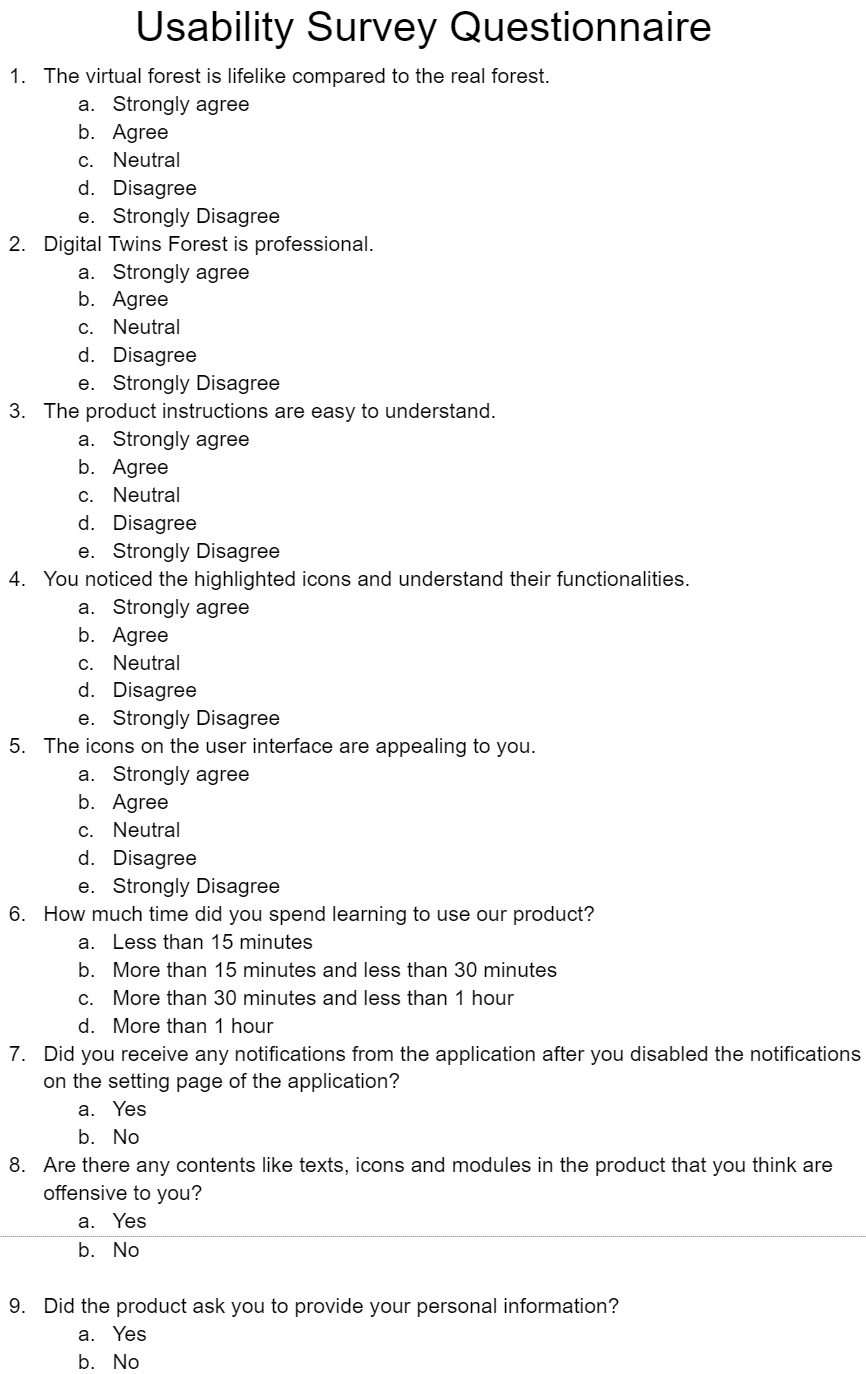
\includegraphics[scale = 0.9]{VnV_Pictures/Usability Survey Quesntionnarie.png}
    \caption{Usability Survey Questionnaire}
\end{figure}

\newpage

\subsection{Pictures}
The following is a sample turn page button:
\begin{figure}[H]
    \centering
    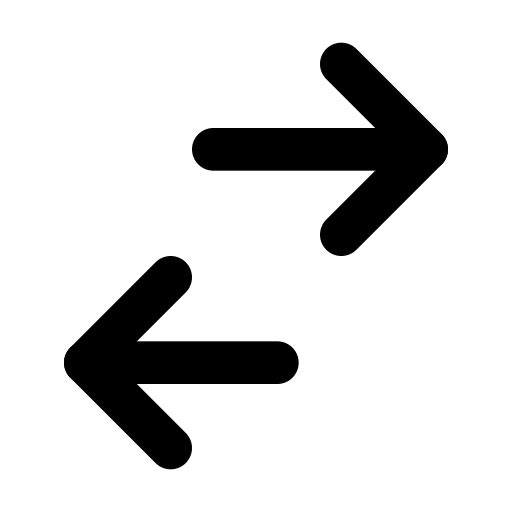
\includegraphics[scale = 0.5]{VnV_Pictures/turnpage_icon.png}
    \caption{Turn Page Button}
\end{figure}

\noindent The following is a sample minimize button:
\begin{figure}[H]
    \centering
    
\includegraphics[scale = 0.5]{VnV_Pictures/tree_parameter.png}
    \caption{Show/Minimize Tree Parameter Data Button}
\end{figure}

\begin{figure}[H]
    \centering
    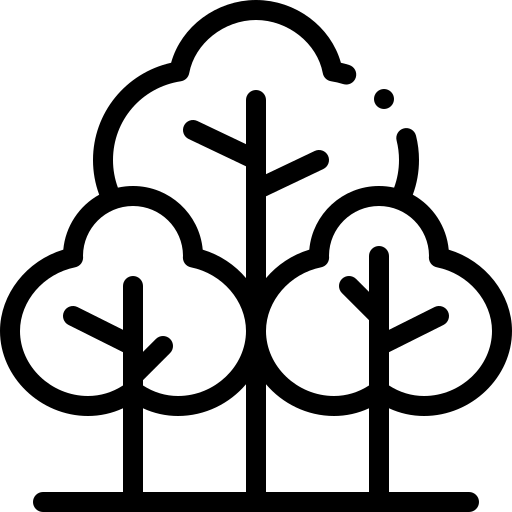
\includegraphics[scale = 0.5]{VnV_Pictures/environmental_data.png}
    \caption{Show/Minimize Environmental Data Button}
\end{figure}

\newpage


\newpage{}
\section*{Appendix --- Reflection}

The information in this section will be used to evaluate the team members on the
graduate attribute of Lifelong Learning.  Please answer the following questions:

\begin{enumerate}
  \item What knowledge and skills will the team collectively need to acquire to
  successfully complete the verification and validation of your project?
  Examples of possible knowledge and skills include dynamic testing knowledge,
  static testing knowledge, specific tool usage etc.  You should look to
  identify at least one item for each team member.
  \item For each of the knowledge areas and skills identified in the previous
  question, what are at least two approaches to acquiring the knowledge or
  mastering the skill?  Of the identified approaches, which will each team
  member pursue, and why did they make this choice?
\end{enumerate}

The knowledge and skills the team need to acquire to complete the verification and validation of our project are listed below:
\begin{itemize}
    \item dynamic testing knowledge
    \item static testing knowledge
    \item automatic and manual testing knowledge
    \item the use of Unity
    \item design of questionnaire and user interview
\end{itemize}

Jiacheng is responsible for dynamic testing knowledge. The possible approaches to acquire it include online tutorials and the experience of the mandatory testing course we took last semester. He decided to pursue this knowledge because it is essential for the validation of the product, and the correctness has to be proved in the process of execution. Furthermore, he is familiar with dynamic testing knowledge.\\

Tingyu is responsible for static testing knowledge. Possible approaches to acquire this kind of knowledge could be the experience of a testing course we took, searching online, discussing in the group and talking to experts. Static testing is significant in the verification process, and it would include technical or informal review, inspection, walkthrough, static code review, etc. As Tingyu is also responsible for organizing regular meetings and taking the script, he would love to study static testing knowledge and put static testing into our meetings as a part of the discussion. He would control and manage the process of static testing.\\

Yichen is responsible for automatic and manual testing knowledge. Knowledge about automatic and manual testing can be gained from the online materials, experience in the testing course, and more. The knowledge of automatic testing will mainly apply to parametric modelling and data storage. And manual testing will be used on the other part, as our product relies on the user interface, and we have to check the overall results manually. Yichen decided to pursue this kind of knowledge because she will take care of the overall effect of the user interface and make modifications along with the testing results. \\

Bowen is responsible for the use of Unity. The possible methods of gaining knowledge of Unity include online tutorials, experience from past courses, and talking to experts. Bowen will work as the main developer for the modelling part and has one year of CO-OP experience working on Unity, and that is why he will pursue this skill.\\

Junhong is responsible for the design of the questionnaire and user interview. The possible approaches to gaining this skill include learning in human-computer interaction class, searching online, and learning about successful cases we can find. This skill is essential because we would love to know how the user feels using our product to get a full view of the usability and user experience. Moreover, this can only be achieved by asking our users. Junhong decided to pursue this one because he already deeply understands this skill and has performed many independent projects with questionnaires. 
\end{document}